\documentclass{article}

\usepackage{amsmath}
\usepackage{float}
\usepackage{csvsimple}
\usepackage{graphicx}
\usepackage{adjustbox}

\usepackage[citestyle=numeric,style=numeric, backend=bibtex8]{biblatex}

\graphicspath{ {../results/} }

\addbibresource{citations.bib}

\begin{document}

  \title{Linear Time Generation and Coloring of Simulated Wireless Sensor Networks Simulated with Random Geometric Graphs}
  \author{Luke Wood}
  \maketitle

  \section{Executive Summary}
	Wireless Sensor Networks (WSNs) are a group of ad hoc wireless devices that communicate amongst themselves.
  WSNs have tons of applications coming in the near future ranging from traffic sensing networks to weather reading sensors on the surface of Mars\cite{mahjoub2010employing}.
	They are incredibly expensive to develop and test which makes them a great candidate for simulation as a preliminary way to gather data.
	Vlady Ravelomananana and Hichem Kenniche from the University of Paris first explored the concept of using random geometric graphs (RGGs) to attempt to model wireless sensor networks \cite{kenniche2010random}.
  At the moment random geographic graphs are the state of the art method for simulating WSNs.
	This project uses RGGs as a way to gather valuable information about how wireless sensor networks will possibly function and communicate.

  \subsection{Introduction and Summary}
	This report generates and analyzes RGGs in the following ways as an attempt to gain some insight into the behavior of wireless sensor networks:
	\begin{enumerate}
		\item Generating RGGs on the geometries of a unit square, unit disc, and unit sphere
		\item Color the generated graph in linear time using smallest vertex last ordering\cite{matula1983smallest}
		\item Find the terminal clique in the generated RGGs
		\item Find a selection of bipartite subgraphs producted by an algorithm for coloring
	\end{enumerate}
	The generation portion of this report generates graphs consisting of N vertices with an average degree of A on the geometric topologies of unit square, unit disc, unit sphere in linear time.
	Some tables are included to display benchmark data for generated RGGs of various size to display the performance of the implementation of the algorithms.

	One interesting thing to notice in the tables is that as the number of nodes grows the real average degree converges on the expected average degree.
	The lower the number of nodes the further from the expected average degree the real number is.
	This happens due to there not being enough nodes in the graph for the real radius to reach the expected value.
  The random error in the point generation is more apparent when there are fewer nodes in the graph.

  The coloring algorithms also run in $O(V+E)$ which is linear time as the edges are capped by the value A which is a constant.
  The runtimes could also be rewritten as $O(V + A*V)$ which is $O(V)$ assuming the A is a constant value.

  \begin{table}
    \label{benchmarks}
    \centering
    \begin{adjustbox}{width=1\textwidth}
    \csvautotabular{../results/benchmarks/full_benchmark.csv}
    \end{adjustbox}
    \caption{Full Benchmark Data Generated, Subsets of this Data Available in Other Tables for Readability}
  \end{table}

  Reference table \ref{benchmarks} for the full benchmarks.

  \subsection{Programming Environment Description}
		The implementation of the algorithm used to gather the data supporting this report was gathered on a 15 inch Macbook pro 2017 with a 2.9 GHz Intel Core i7 processor and 16 GB of RAM.
		The computer is running macOS High Sierra.
    The python environment is used for the ability to leverage the networkx library for plotting graphs as well as matplotlib to easily create charts.
    The algorithms are implemented to run in linear time and despite pythons low speed still run in reasonable time spans even on large input sizes.

    The generation as well as coloring algorithms were both implemented again in the Elixir programming language, however this proved problematic as all data structures are immutable.
    On small inputs, the Elixir implementation ran up to 5 times as fast as the python implementation, however there is no data structure with $O(1)$ insertion, access, and deletion in Elixir.
    The best runtime possible in pure Elixir was $O(n*log(n))$ which was worse than the python version.
    This made it impossible to implement the coloring algorithm in linear time without interopping with C or Erlang.
    Due to time constraints, it was not feasible to get the interop working with Erlang or C in time.
    Thus the implementation is still in python, however if I could do it again I would either follow through with the Erlang interop and continue in Elixir or use a different platform entirely.

  \section{Reduction to Practice}
    This section will describe the transition from theory to implementation.
    This section will also give a detailed analysis of the algorithms used in this project as well as their asymptotic runtimes.
	\subsection{Data Structure Design}
		The generation portion of this project uses several different data structures.
		The first one is a python object of custom type node.
		This serves as a tuple of values consisting of a list of dimensions, a list of nodes, and a node number.
		The first two are used during graph generation and the latter during conversion to an adjacency list.
		This data structure could be used interchangeably with a statically indexed tuple instead of an object to avoid any overhead associated with objects in python, however the readability gained from using a custom node class heavily outweighs the marginal performance benefit gained from using a statically indexed tuple.
		Both of these data structures provide $O(1)$ read and write operations.
    The python wiki states that dictionary access time is amortized $O(1)$, however in the worst case can be $O(n)$\cite{pythonwikiruntimes}.
    That being said, most interpreters will convert objects with known attributes into statically indexed arrays so it is likely that there would be neglible performance difference anyways.
		If the goal were to generate gigantic graphs then an argument could be made to switch over the statically indexed tuples to reduce the access time for attributes by a bit as tuples use static memory address offsets.

		The second data structure used in the implementation is the adjacency list.
		Adjacency lists are an efficient graph representation that we will use in the subsequent reports.
		Adjacency lists require only $O(V+E)$ storage as opposed to the $O(v^2)$ required for adjacency matrixes.
    Despite the huge potential savings on storage, the only sacrifice adjacency lists make is in the lookup operation to determine if there is an edge between two nodes.
    The sacrifice made in adjacency lists is $O(A)$ lookup time for the existence of an edge as opposed to $O(1)$ lookup time available in adjacency matrixes.
		This makes adjacency lists useful in situations where the expected average number of edges is significantly lower than the number of nodes in the graph.

    In the coloring portion of the project, I used the same data structures above as well as a hash set.
    When I am keeping track of which nodes are of degree n, I frequently have to move each node's neighbors down a degree.
    In order to get optimal big O, I needed to use a data structure with constant time access, constant time add, and constant time deletion.
    Hash set seemed like a perfect match for the problem at hand as we only needed to know of each member was a set.
    In python, sets have amortized $O(1)$ runtime for all three of the aforementioned operations\cite{pythonwikiruntimes}.

	\subsection{Algorithm Description}
		This section gives a detailed analysis of the algorithms used in the graph generation, graph coloring, and backbone selection.

  \paragraph{Square Point Generation}
		The algorithm to generate the points in the unit square topology is simple.
		The steps are as follows:
    \begin{enumerate}
      \item x=random(0, 1), y=random(0, 1)
      \item add (x,y) to a list of points
      \item repeat steps 1 and 2 until N points are created
    \end{enumerate}
    That is all that is necesary to get a random point in the unit square.
    This algorithm is $\Theta(n)$.

  \paragraph{Disc Point Generation}
		Generating the points on the disc topology is slightly more challenging than generating the points for the square topology.
    The algorithm for generating points used in the implementation descriped in this point is as follows:
    \begin{enumerate}
      \item x=random(0, 1), y=random(0,1)
      \item if the distance from (x,y) to (.5, .5) is < .5, add (x,y) to a list of points
      \item repeat steps 1 and 2 until N points are created
    \end{enumerate}
    The issue with this algorithm is the nondeterminism involved in creating each point.
    When generating large numbers of points lots of work is wasted on generating the unused random points.
    In future iterations of this project a mathematical approach may be used to generated these points.
    Despite the non-determinism, this algorithm is still amortized $\Theta(n)$.

    A possible approach to fixing this implementation would be to pick a radius between 0 and 1, and then rotate by a random number of radians between 0 and 2$\pi$.
    This was not implemented as I was unsure if this would produce a uniform distribution.

    This is not pure $O(n)$ as due to the non-determinism it could theoretically run indefinitely.
    This is however of lower probability than flipping a coin repeateadly and getting heads for all eternity.

  \paragraph{Sphere Point Generation}
    Generating points on the surface of the unit sphere can be solved using math.
    The steps for the following algorithm are as follows:

    \begin{enumerate}
      \item u = (random() * 2) - 1, theta = random() * 2 * pi
      \item x = sqrt(1 - u**2) * cos(theta), y = sqrt(1 - u**2) * sin(theta), z = u
      \item append (x, y, z) to a list of points.
      \item repeat steps 1-3 N times
    \end{enumerate}

    In the implementation associated with this report the values x, y, and z are transformed to form a sphere around (.5, .5, .5) as opposed to (0, 0, 0) as it makes the connection algorithm simpler.
    This algorithm is $\Theta(n)$.

	\subsection{Node Connection}
		In order to ensure that average degree of the nodes is close to the desired average degree, a radius of a specific length can be defined surrounding each node.
    The nodes within that radius of each other are then connected in the graph.
		The formulas to find the radius for each topology is derived from the equations found in the paper Bipartite Grid Partitioning of a Random Geometric Graph\cite{chen2017bipartite}.
		The formula used to find this radius varies for each graph tolopogy and can be found in the table \ref{radius_equations}.

    \begin{table}
      \centering
      \label{radius_equations}
  		\begin{tabular}{ |c|c|c| }
  				\hline
  				Topology &  Radius Equation \\
  				\hline
  				Unit Square & $r = sqrt(\dfrac{d(G)}{N\pi})$ \\
  				\hline
  				Unit Disc & $r = sqrt(\dfrac{d(G)}{N})$ \\
  				\hline
  				Unit Sphere & $r = sqrt(\dfrac{2*d(G)}{N})$ \\
  				\hline
  		\end{tabular}
    \end{table}

    The brute force algorithm for generating and connecting RGGs in this way is $O(n^2)$.
    This quickly became problematic as the algorithm took upwards of 200 seconds to run on input size of only 12,000.
    Figure \ref{brute_force_runtimes} shows this issue.
    \begin{figure}
      \centering
      \label{brute_force_runtimes}
      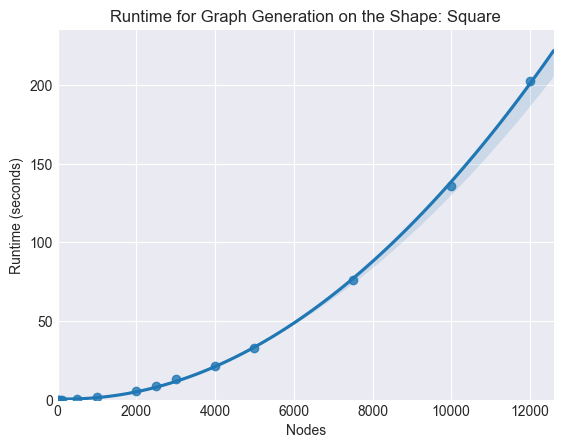
\includegraphics[width=1 \textwidth]{square/generation/runtime/runtime_chart_naive}
      \caption{Runtimes of the $O(n^2)$ Algorithm}
    \end{figure}
    Instead, the implementation uses a bucket method to narrow down the required number of comparisons.
    The idea for this algorithm comes from the paprer Bipartite Grid Partitioning of a Random Geometric Graph\cite{chen2017bipartite}.
    The algorithm can be broken down into steps as follows:

    \begin{enumerate}
      \item create $(\sqrt{1/R} - 1 )^2$ buckets
      \item place buckets in a 2D grid arrangement
      \item for each node, place the node in bucket (x, y) such that x=$floor(x*num_buckets)$, y=$floor(y*num_buckets)$
      \item for each x,y such that x=0..buckets, y=0..buckets
      \item check to see if each node in bucket (x,y) is within radius R to all others in bucket (x,y) as well as (x+1,y-1), (x+1,y), (x,y+1), (x+1,y+1)
      \item if two nodes are under radius R from each other, place an edge between them.
    \end{enumerate}
    This algorithm is $O(n)$ given a small enough radius and a sufficient number of buckets.
    This means that with sufficiently many nodes and as long as the expected average degree remains low the algorithm will be linear.
    The runtimes for the implementation of this algorithm can be found in figure \ref{optimised_runtimes_for_connection}.
    \begin{figure}
      \centering
      \label{optimised_runtimes_for_connection}
  		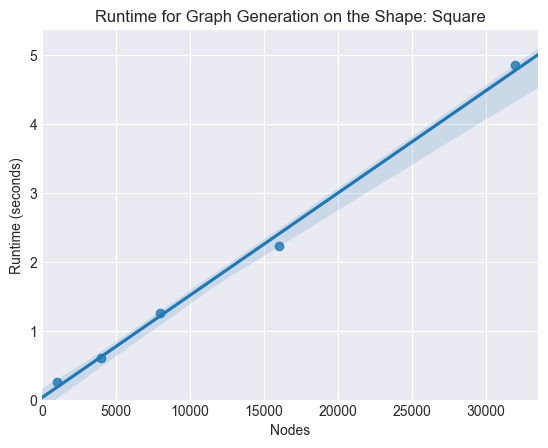
\includegraphics[width=1 \textwidth]{square/generation/runtime/runtime_chart}
  		\caption{Runtimes of the $O(n)$ Algorithm}
	  \end{figure}

  \paragraph{Shortest Last Vertex Ordering}
    In order to color the graph in linear time, the shortest last vertex ordering is used as a heuristic to get a reasonable coloring of the graph.
    To compute the ordering in $O(V+E)$ time, the following algorithm is used.
    Graphics are attached to visualize each step of the process.

    To begin the graph is uncolored, this can be seen in figure \ref{uncolored_graph}.
    The next step is to initialize the ordering of the nodes.
    To do so, the following data structures are created:
    \begin{enumerate}
      \item A map mapping from degrees to nodes which are of that degree.
      \item Each item mapped to in the previous map should be a set.
      \item A map mapping from node numbers to the degree of that node.
    \end{enumerate}
    Then, the following steps are executed for N iterations:
    \begin{enumerate}
      \item Select a node from a non-empty set mapped to by the smallest possible degree
      \item Add this node to the ordering
      \item Remove the node from the graph, this entails decrementing the degree of all neighbors and removing the node from the sets above.
      \item Move all of the neighboring nodes one hash set lower in the map mapping from degree to nodes
    \end{enumerate}
    Figure \ref{ordering_graph} shows this process for a graph with 20 nodes.
    After the ordering is complete, the ordering is then used to color the graph.

    \begin{figure}
      \centering
      \label{uncolored_graph}
      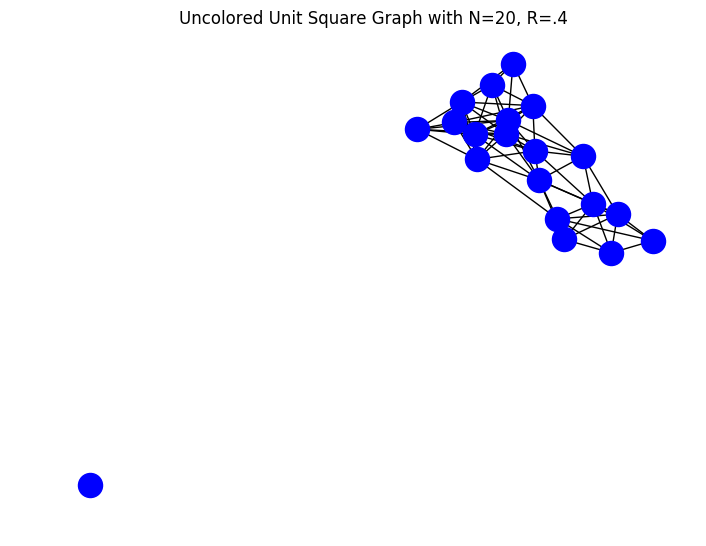
\includegraphics[width=1 \textwidth]{walkthrough/uncolored}
      \caption{An Uncolored Graph on the square topology of N=20, and R=.4}
    \end{figure}

    \begin{figure}
      \centering
      \label{ordering_graph}
      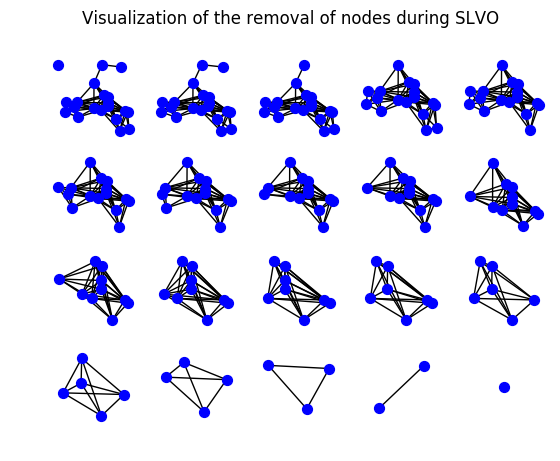
\includegraphics[width=1 \textwidth]{walkthrough/ordering}
      \caption{An Example of Shortest Vertex Last Ordering}
    \end{figure}

    \paragraph{Graph Coloring}
    The coloring process is rather simple.
    Each node is taken from the ordering and is given the smallest color not yet assigned to any of it's neighbors.
    This is repeated until all nodes are colored.
    Figure \ref{coloring_graph} shows this process for the same example above.
    After this is complete, the graph will be fully colored.
    Figure \ref{colored_graph} shows a fully graphed graph.

    \begin{figure}
      \centering
      \label{coloring_graph}
      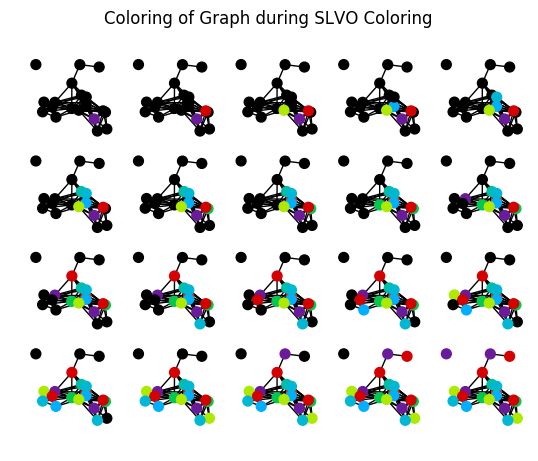
\includegraphics[width=1 \textwidth]{walkthrough/coloring}
      \caption{The Process of Coloring the Graph using SVLO}
    \end{figure}

    \begin{figure}
      \centering
      \label{colored_graph}
      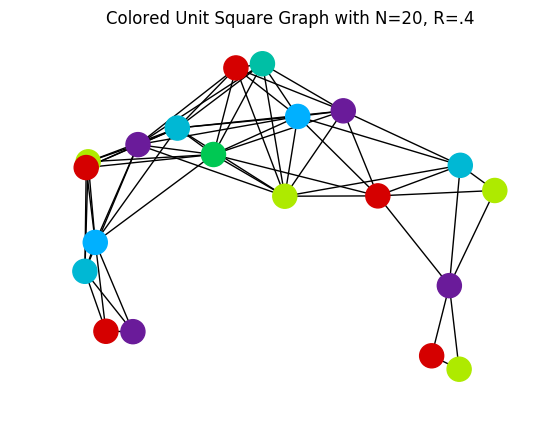
\includegraphics[width=1 \textwidth]{walkthrough/final_colored}
      \caption{A Fully Colored Graph}
    \end{figure}

    \paragraph{Backbone Selection}
    After the graph coloring is completed, the next thing done is selecting the communication backbone.
    This is done by first selecting the four largest color sets produced from the coloring above.
    Then, the backbone is created for each of the 6 combinations of the four colors.
    Each backbone consists of each node in the two selected colors.
    Six backbones from the coloring example above are included in figure \ref{six_backbones}.

    \begin{figure}
      \centering
      \label{six_backbones}
      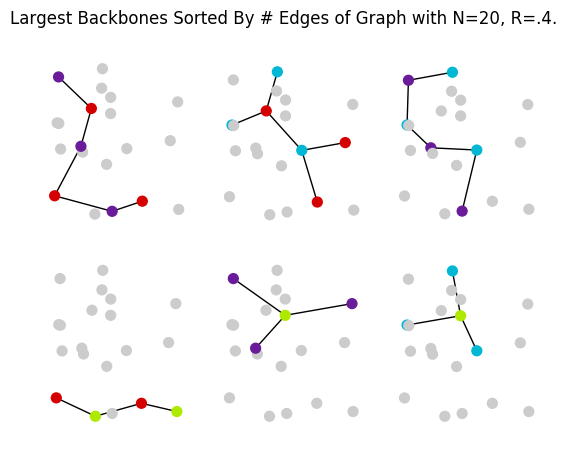
\includegraphics[width=1 \textwidth]{walkthrough/largest_backbones}
      \caption{The Six Largest Backbones for a graph with N=20, R=.4}
    \end{figure}

    In order to compute the domination of the backbones, an empty set is initialized.
    Then, for each edge in the backbone both nodes are added to the set.
    After all the edges are traversed the size of the set divided by N is the domination of the backbone.

    All of these algorithms can be implemented in linear time trivially given the proper data structure selections.

  \subsection{Algorithm Engineering}
    \paragraph{Graph Generation}
    As mentioned above, the brute force algorithm to find adjacent nodes becomes slow at a fast rate.
    To fix this, the implementation presented uses linear time algorithms for all of it's operations.
	  Table \ref{runtime_comparison_table_brute} compares the runtimes of the linear implementation to that of the quadratic implementation.

	  \begin{table}
      \centering
      \label{runtime_comparison_table_brute}
  		\begin{tabular}{ |c|c|c| }
  			\hline
  			Nodes & $O(n^2)$ & $O(n)$ \\
  			\hline
  			  1000 & 0.258400 & 0.657174 \\
  			  \hline
  			  2000 & 0.382116 & 2.630040 \\
  			  \hline
  			  3000 & 0.473916 & 5.874501 \\
  			  \hline
  			  5000 & 0.831753 & 16.809004 \\
  			  \hline
  			  10000 & 1.560216 & 65.398991 \\
  			\hline
  		\end{tabular}
  		\caption{Runtimes of the $O(n)$ and $O(n^2)$ algorithms for generating graphs}
	  \end{table}

	  The $O(n)$ algorithm is far superior even on small input sizes such as 1000.
    The final implementation uses $O(n)$ time as well as $O(n*A)$ space where A=aveage edge density.
    This is accomplished by ensuring that each node is stored in a representation that only references adjacent edges.
    The implementation also only compares nodes to nodes in adjacent buckets to determine if an edge should be placed between them.
    Each node only has at most $5nr^2$ comparisons\cite{chen2017bipartite}.
    With reasonably spare graphs this maintains a runtime of $O(n)$ however with large enough radii this can begin to behave like $O(n^2)$.
    This yields an $O(n)$ time and $O(n)$ space on the type of inputs this implementation targets.

    \paragraph{Shortest Last Vertex Ordering}
    The SLVO algorithm used in this paper is an $O(V+E)$ algorithm.
    This section describes the implementation of the shortest last vertex ordering algorithm described in the previous section.
    The first step is the initialization.
    Table \ref{used_structures_slvo} shows the data structures and access times for the data structures used.
    All of these runtimes are confirmed by the official python documentation\cite{pythonwikiruntimes}.
    Please note some of these runtimes are amortized, in the worst case many of these operations are $O(n)$.

    \begin{table}
      \centering
      \label{used_structures_slvo}
      \begin{tabular}{ |c|c|c|c|c| }
        \hline
        Requirement & Data Structure & Access Time & Insertion Time & Deletion Time \\
        \hline
        Degree to set of Nodes & Dictionary & $O(1)$ & $O(1)$ & $O(1)$ \\
        \hline
        Set of Nodes & Set & $O(1)$ & $O(1)$ & $O(1)$ \\
        \hline
        Node to Degree & Dictionary & $O(1)$ & $O(1)$ & $O(1)$ \\
        \hline
        Ordering & Python List(Array) & $O(1)$ & $O(1)$ & $O(N)$ \\
        \hline
      \end{tabular}
      \caption{Data Structures Used in the Initialization for SLVO}
    \end{table}

    After the initialization step, we move into the meat of the algorithm.
    The steps are run the same was as described in the algorithm
    Table \ref{big_o_slvo} describes the big O of each step when using the data structures used above.

    \begin{table}
      \centering
      \label{big_o_slvo}
      \begin{tabular}{ |c|c| }
        \hline
        Select a node from a non-empty set mapped to by the smallest possible degree & $O(1)$ \\
        \hline
        Add this node to the ordering & $O(1)$ \\
        \hline
        Remove the node from the graph & $O(1)$ \\
        \hline
        Decrement all neighboring nodes one degree & $O(max(E))$ \\
        \hline
      \end{tabular}
      \caption{Big O of Each Step}
    \end{table}

    The steps in the table run \textit{V} times.
    While it may look like this is $O(V*E)$ due to the last step being $O(E)$, this is not the case as we only traverse each edge once and then remove the nodes.

    \paragraph{Graph Coloring}
    The graph coloring algorithm is also $O(V+E)$.
    To implement the algorithm, I used the following.
    First, a map is initialized from nodes to colors.
    I used a list of size \textit{N} to get constant time access and update as well as to avoid the overhead required to use a hash table.
    All of the values in the coloring have an initial color of -1.
    For each node in the ordering, I select all of the neighbors from the adjacency list.
    I then select the colors at the index of each neighbor and place them into a hash set.
    I then try each color from 0 until there is a color not in the hash set and assign that color to the node.
    Due to the use of the hash set, each color check is $O(1)$.

    Overall, this yields $O(V+E)$ runtime.

    \paragraph{Backbone Selection}
    The only meaningful data structure choice in the backbone selection is the data structure used to represent the set during domination calculation.
    A hash set is a great choice for this.
    The built in set data structure in python has $O(1)$ insertion which is all that is needed for this algorithm.
    By doing this, all of the algorithms required for backbone selection can run in $O(V+E)$.

	\subsection{Verification}
		One way that we verified our results was checking the distribution of edge densities in our graph.
		We expect to see a gaussian distribution in the edge densities with the center being around our calculated radius.
		We can also verify the runtime of our algorithms by plotting the input size on the x axis and the runtime on the y axis.
		If we have a linear algorithm we should be able to fit the distribution of points to a linear equation with minimal error.
		Both of these verification methods were successful and can be seen in the results section of this report.

  \paragraph{Visualizing the Points}
    One way to validate that the points are distributing correctly is by plotting out the points in a scatter plot.
    Early on the implementation had a bug where the points distributed around the radius of the unit disc instead of evenly inside the unit disc.
    Using a scatter plot made this trivial to spot.

    Figure \ref{drawing_of_square} shows the distribution on the square topology,
    Figure \ref{drawing_of_disc} shows the distribution on the disc topology,
    and Figure \ref{drawing_of_sphere} shows the distribution on the sphere topology.
    \begin{figure}
      \centering
      \label{drawing_of_square}
      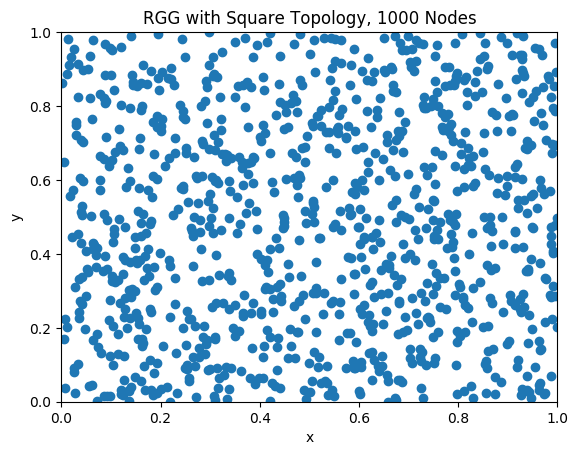
\includegraphics[width=1 \textwidth]{square/generation/drawing/nodes.png}
      \caption{1000 Points on the Square Topology}
    \end{figure}

    \begin{figure}
      \centering
      \label{drawing_of_disc}
      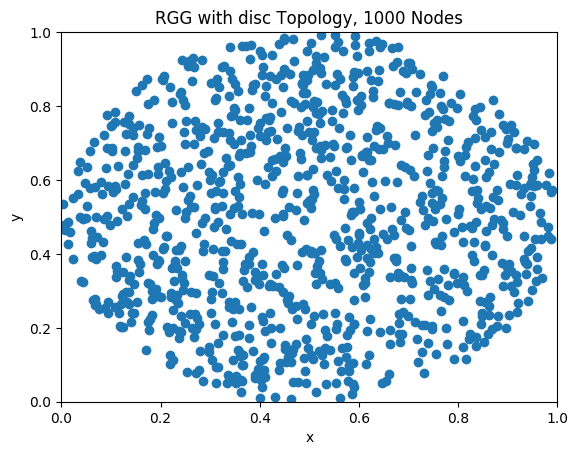
\includegraphics[width=1 \textwidth]{disc/generation/drawing/nodes.png}
      \caption{1000 Points on the Disc Topology}
    \end{figure}
    \begin{figure}
      \centering
      \label{drawing_of_sphere}
      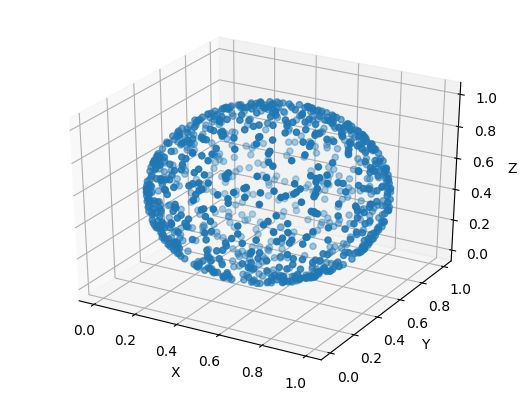
\includegraphics[width=1 \textwidth]{sphere/generation/drawing/sphere_drawing.png}
      \caption{1000 Points on the Sphere Topology}
    \end{figure}

    \paragraph{Edge Density}
    Checking the distribution of the edge densities is one way to verify that the edges are connecting as expected
    The edge distributions should follow a gaussian distribution.
    Figures \ref{square_edge_density}, \ref{disc_edge_density}, and \ref{sphere_edge_density} all show gaussian distrubutions for their respective topologies.
    All of the edge density distributions follow a gaussian distribution which is what is expected meaning that the edges likely connected the nodes in the expected way.

    \begin{figure}
      \centering
      \label{square_edge_density}
      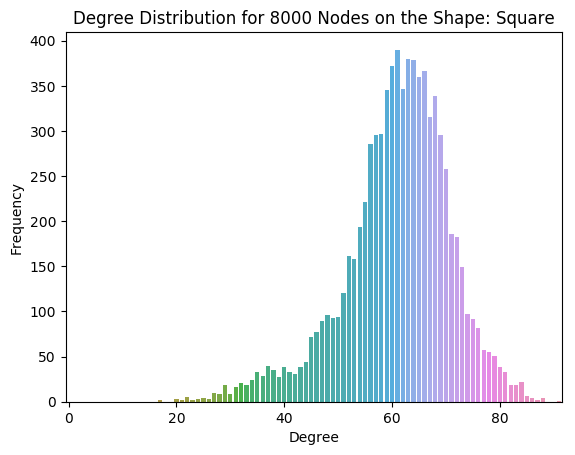
\includegraphics[width=1 \textwidth]{square/generation/edge_density/8000_64.png}
      \caption{Edge Densities of an 8000 Node Graph with E(Degree)=64 on Topology Square}
    \end{figure}

    \begin{figure}
      \centering
      \label{disc_edge_density}
      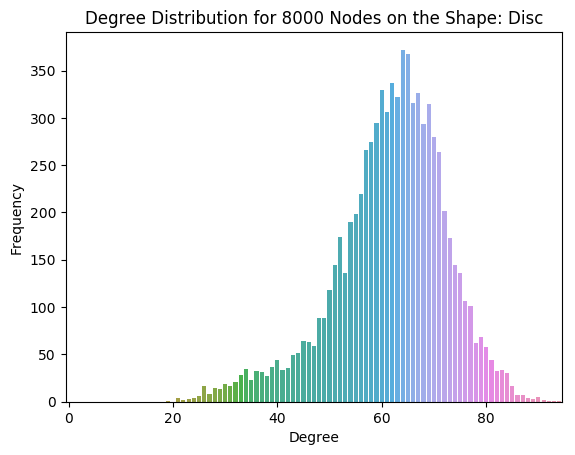
\includegraphics[width=1 \textwidth]{disc/generation/edge_density/8000_64.png}
      \caption{Edge Densities of an 8000 Node Graph with E(Degree)=64 on Topology Disc}
    \end{figure}

    \begin{figure}
      \centering
      \label{sphere_edge_density}
      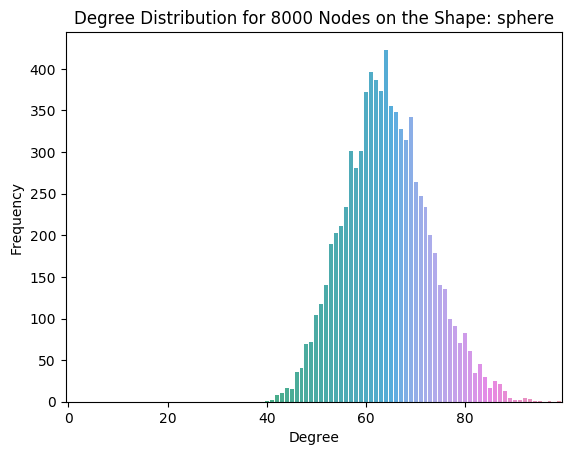
\includegraphics[width=1 \textwidth]{sphere/generation/edge_density/8000_64.png}
      \caption{Edge Densities of an 8000 Node Graph with E(Degree)=64 on Topology Sphere}
    \end{figure}

    \paragraph{Ordering}
    A plot displaying the degrees of the graph against the degrees of nodes when they are removed from the graph during shortest last vertex ordering can be used to make sure the ordering process is behaving as expected.
    Figure \ref{ordering_removal_degrees} shows the expected behavior.
    Both of the plots follow a normal distribution.
    The degrees when removed having a much lower standard deviation along with a lower average.
    The degrees when the graph is generated have a higher standard deviation and a higher average.
    This is the expected result.

    \begin{figure}
      \centering
      \label{ordering_removal_degrees}
      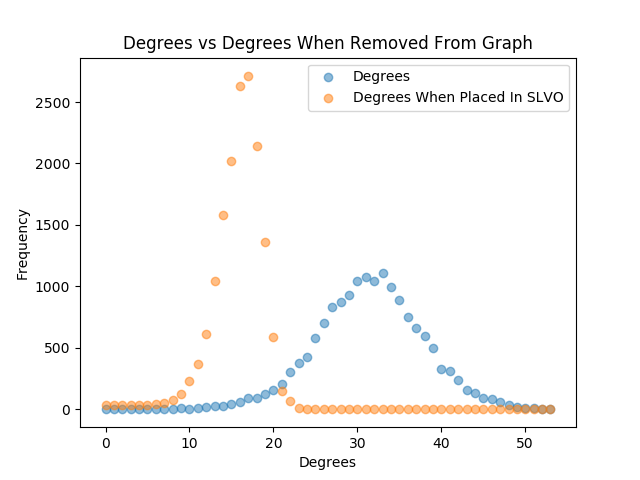
\includegraphics[width=1 \textwidth]{disc/coloring/degree_frequencies.png}
      \caption{Degree Densities when Nodes are Removed During Shortest Vertex Last Ordering}
    \end{figure}

    \paragraph{Coloring}
    To verify that the coloring was working properly we can plot the size of the colors in the graph.
    Figure \ref{color_size_distribution} shows the distribution of the size of each color.
    It makes sense that the earlier colors are used more given that the algorithm assigns the lowest possible color to each node.

    \begin{figure}
      \centering
      \label{color_size_distribution}
      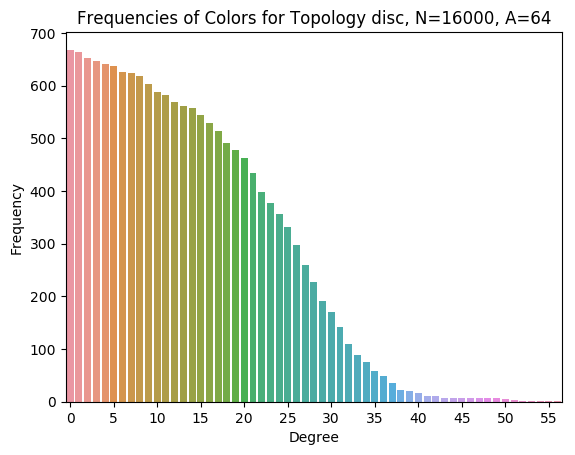
\includegraphics[width=1 \textwidth]{disc/coloring/color_distribution.png}
      \caption{Distribution of the Size of Colors Used}
    \end{figure}

    Some benchmark data related to the graph coloring is included in table \ref{coloring_benchmarks}.

    \begin{table}
      \centering
      \label{coloring_benchmarks}
  	  \csvautotabular{../results/benchmarks/coloring_benchmarks.csv}
  	  \caption{Comparison of Runtimes of Generating the Different Topologies}
    \end{table}

    \paragraph{Shortest Vertex Last Ordering vs Random Ordering}
    In order to further sell the implementation, I have plotted the number of colors used against various values of N for both shortest last vertex ordering and random ordering.
    Both of these algorithms run in linear time.
    Figure \ref{random_coloring_vs_slvo} shows this comparison.
    It is clear that slvo is superior in terms of colors used.

    \begin{figure}
      \centering
      \label{random_coloring_vs_slvo}
      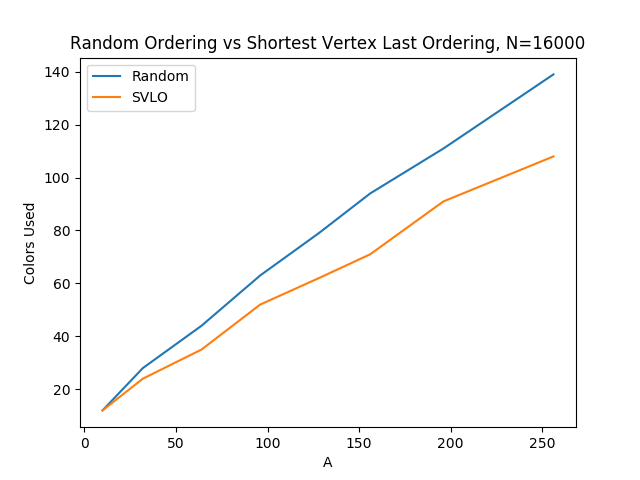
\includegraphics[width=1 \textwidth]{comparison/number_colors.png}
      \caption{Random Order Coloring vs Shortest Last Vertex ordering}
    \end{figure}

    \paragraph{Backbone}
    In order to verify that the backbones were being selected correctly, the top two backbones from each benchmark have been included in this report.


    \begin{figure}
      \centering
      \label{backbone_32_1000_Square}
      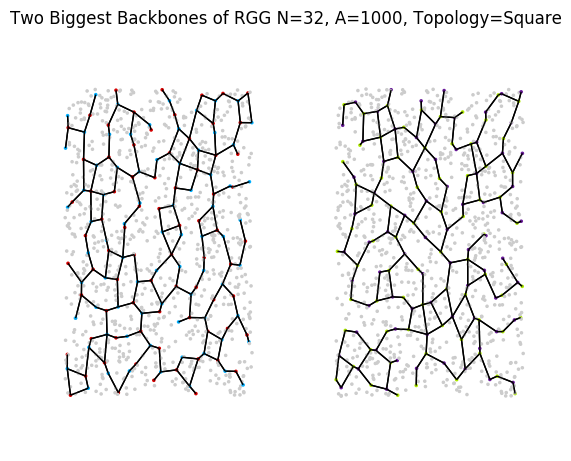
\includegraphics[width=1 \textwidth]{backbone/backbone_32_1000_Square.png}
      \caption{Top Two Backbones, N=1000, A=32, Topology Square}
    \end{figure}

    \begin{figure}
      \centering
      \label{backbone_32_16000_Square}
      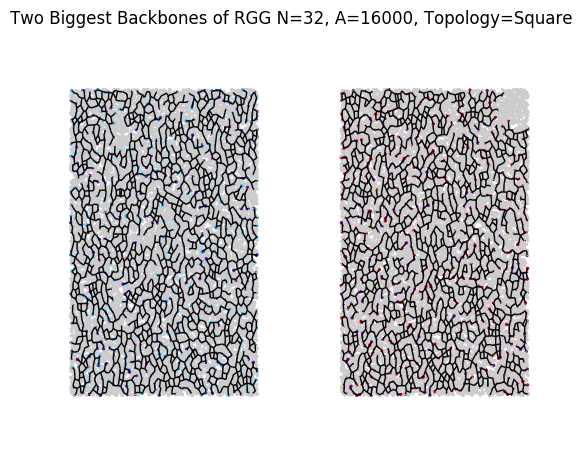
\includegraphics[width=1 \textwidth]{backbone/backbone_32_16000_Square.png}
      \caption{Top Two Backbones, N=16000, A=32, Topology Square}
    \end{figure}

    \begin{figure}
      \centering
      \label{backbone_64_8000_Disc}
      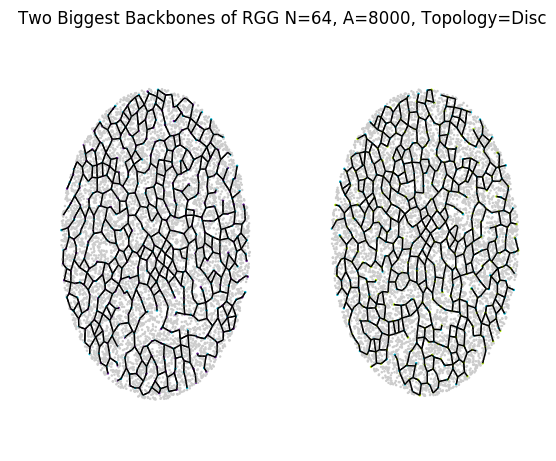
\includegraphics[width=1 \textwidth]{backbone/backbone_64_8000_Disc.png}
      \caption{Top Two Backbones, N=8000, A=64, Topology Disc}
    \end{figure}

    \begin{figure}
      \centering
      \label{backbone_64_8000_Square}
      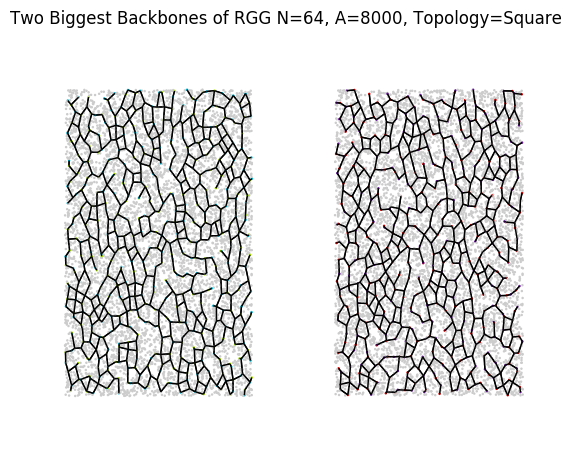
\includegraphics[width=1 \textwidth]{backbone/backbone_64_8000_Square.png}
      \caption{Top Two Backbones, N=8000, A=64, Topology Square}
    \end{figure}

    \begin{figure}
      \centering
      \label{backbone_64_16000_Sphere}
      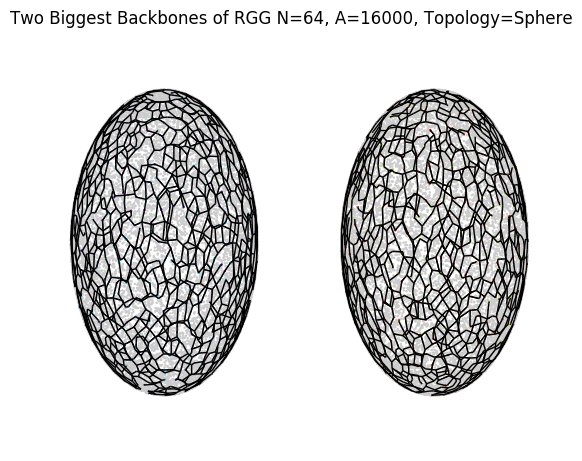
\includegraphics[width=1 \textwidth]{backbone/backbone_64_16000_Sphere.png}
      \caption{Top Two Backbones, N=16000, A=64, Topology Sphere}
    \end{figure}

    \begin{figure}
      \centering
      \label{backbone_64_64000_Disc}
      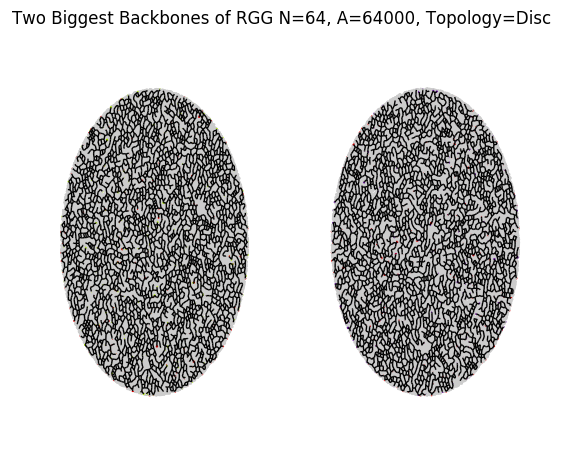
\includegraphics[width=1 \textwidth]{backbone/backbone_64_64000_Disc.png}
      \caption{Top Two Backbones, N=64000, A=64, Topology Disc}
    \end{figure}

    \begin{figure}
      \centering
      \label{backbone_64_64000_Square}
      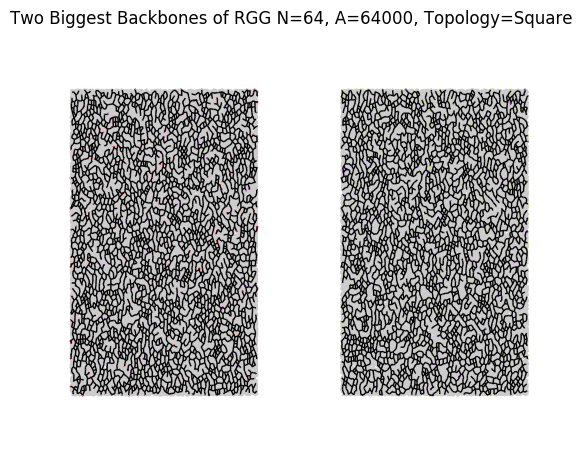
\includegraphics[width=1 \textwidth]{backbone/backbone_64_64000_Square.png}
      \caption{Top Two Backbones, N=64000, A=64, Topology Square}
    \end{figure}

    \begin{figure}
      \centering
      \label{backbone_64_128000_Square}
      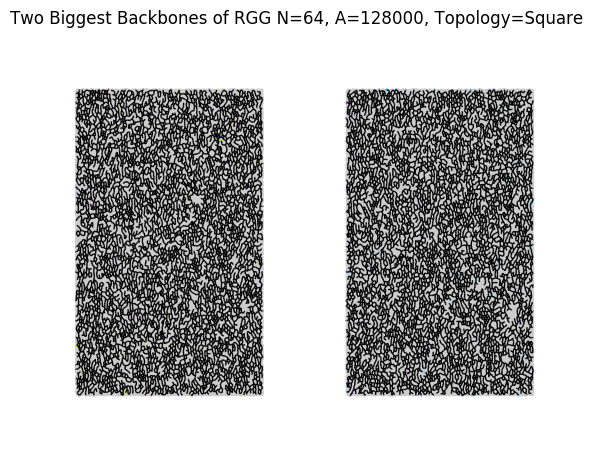
\includegraphics[width=1 \textwidth]{backbone/backbone_64_128000_Square.png}
      \caption{Top Two Backbones, N=128000, A=64, Topology Square}
    \end{figure}

    \begin{figure}
      \centering
      \label{backbone_128_32000_Sphere}
      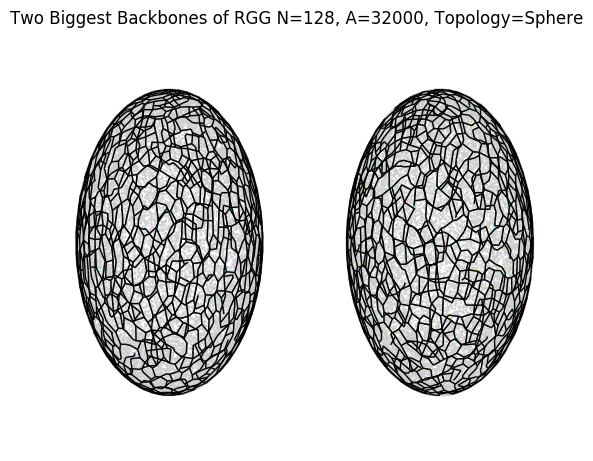
\includegraphics[width=1 \textwidth]{backbone/backbone_128_32000_Sphere.png}
      \caption{Top Two Backbones, N=32000, A=128, Topology Sphere}
    \end{figure}

    \begin{figure}
      \centering
      \label{backbone_128_64000_Disc}
      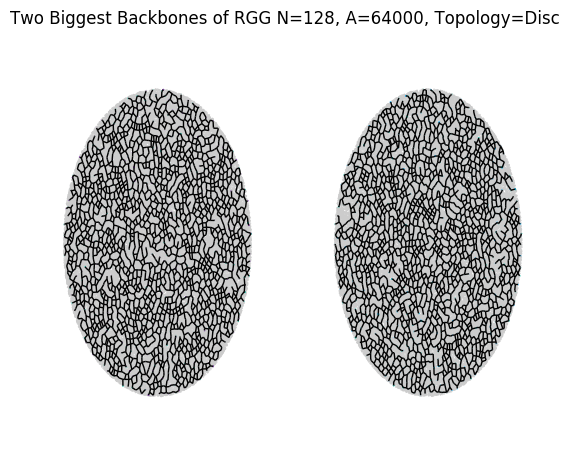
\includegraphics[width=1 \textwidth]{backbone/backbone_128_64000_Disc.png}
      \caption{Top Two Backbones, N=64000, A=128, Topology Disc}
    \end{figure}

    \begin{figure}
      \centering
      \label{backbone_128_64000_Sphere}
      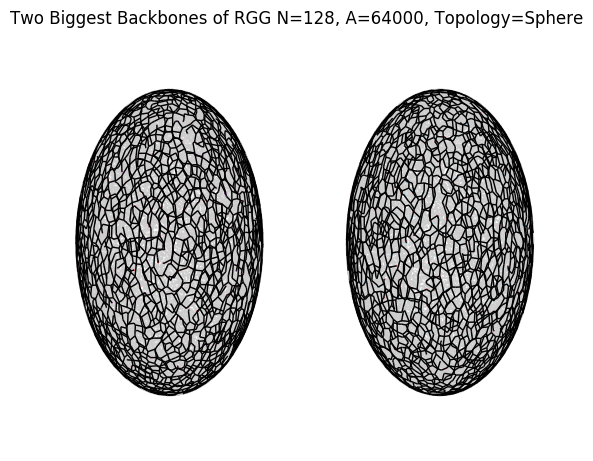
\includegraphics[width=1 \textwidth]{backbone/backbone_128_64000_Sphere.png}
      \caption{Top Two Backbones, N=64000, A=128, Topology Sphere}
    \end{figure}

    \begin{figure}
      \centering
      \label{backbone_128_64000_Square}
      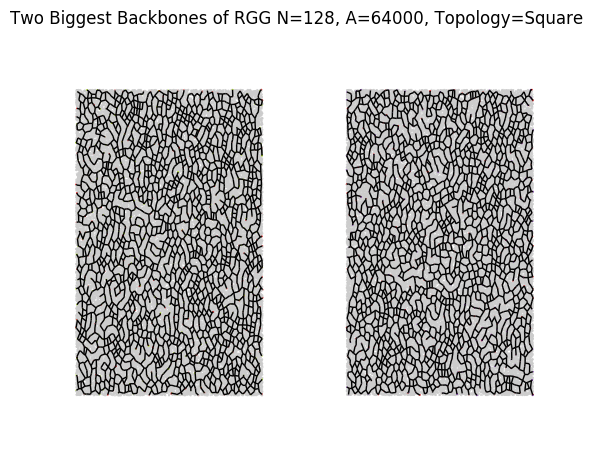
\includegraphics[width=1 \textwidth]{backbone/backbone_128_64000_Square.png}
      \caption{Top Two Backbones, N=64000, A=128, Topology Square}
    \end{figure}

    \begin{figure}
      \centering
      \label{backbone_128_128000_Square}
      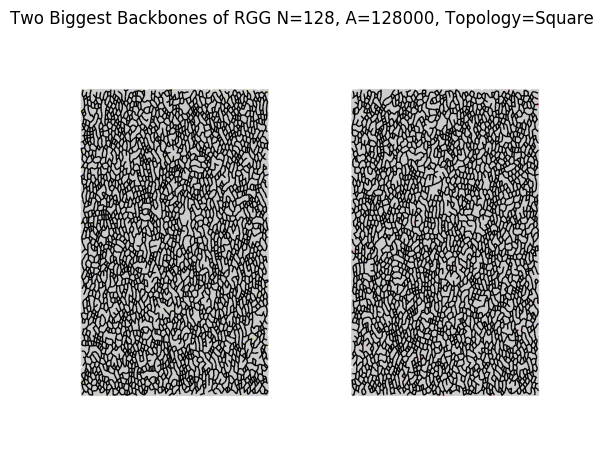
\includegraphics[width=1 \textwidth]{backbone/backbone_128_128000_Square.png}
      \caption{Top Two Backbones, N=128000, A=128, Topology Square}
    \end{figure}

\section{Result Summary}
  All of my algorithms ran in $O(n)$ time.
  There was variance between the runtime of the different topologies due to the way the points were generated combined with the calculation required to compute 2d distance vs 3d distance.
  Table \ref{runtime_comparison_by_topology} shows the runtime of all of the topologies in a table.
  Figures \ref{square_rgg_runtime_chart}, \ref{disc_rgg_runtime_chart}, and \ref{sphere_rgg_runtime_chart} show the individual runtime charts.
  Figure \ref{all_rgg_runtimes_chart} shows all of the runtimes of the different RGG generation algorithms overlaying each other.
  As discussed in the verification section, multiple plots have been used to verify the accuracy of the algorithms.

  \begin{table}
    \centering
    \label{runtime_comparison_by_topology}
	  \csvautotabular{../results/shared/generation/generation_speeds.csv}
	  \caption{Comparison of Runtimes of Generating the Different Topologies}
  \end{table}

  \begin{figure}
    \centering
    \label{square_rgg_runtime_chart}
    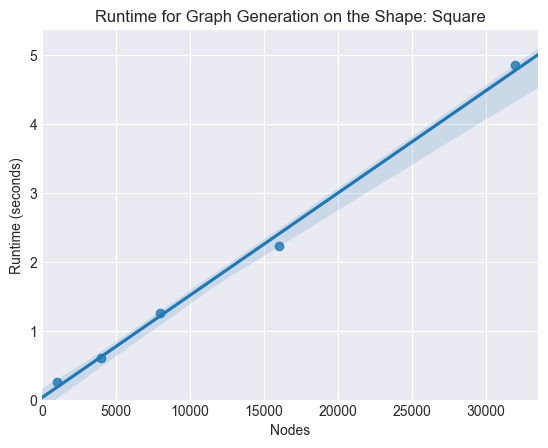
\includegraphics[width=1 \textwidth]{square/generation/runtime/runtime_chart}
    \caption{Runtimes of the $O(n)$ Square RGG Generation Algorithm}
  \end{figure}

  \begin{figure}
    \centering
    \label{disc_rgg_runtime_chart}
    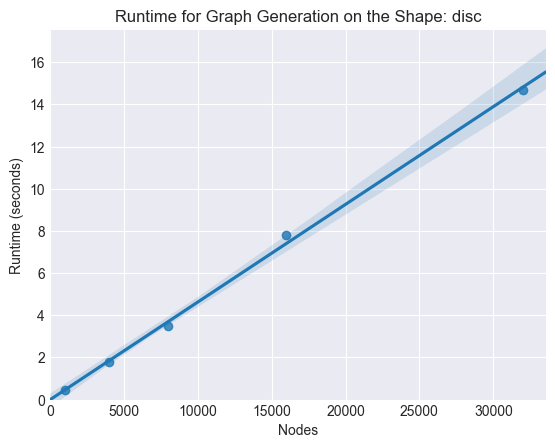
\includegraphics[width=1 \textwidth]{disc/generation/runtime/runtime_chart}
    \caption{Runtimes of the $O(n)$ Disc RGG Generation Algorithm}
  \end{figure}

  \begin{figure}
    \centering
    \label{sphere_rgg_runtime_chart}
    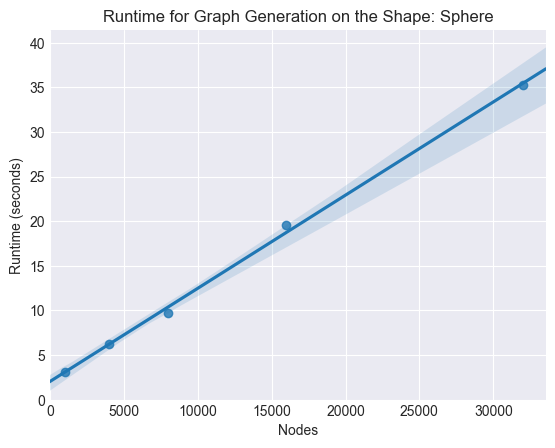
\includegraphics[width=1 \textwidth]{sphere/generation/runtime/runtime_chart}
    \caption{Runtimes of the $O(n)$ Sphere RGG Generation Algorithm}
  \end{figure}

  \begin{figure}
    \centering
    \label{all_rgg_runtimes_chart}
    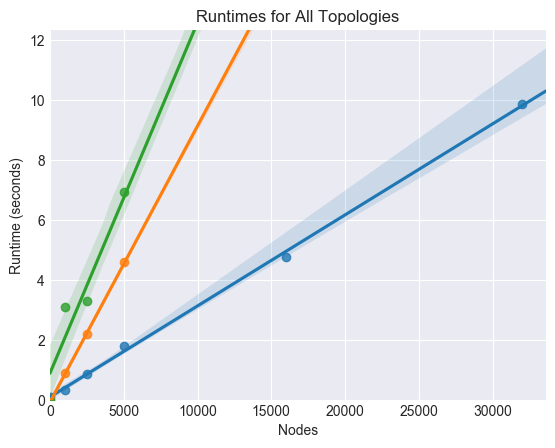
\includegraphics[width=1 \textwidth]{shared/generation/runtime/running_times}
    \caption{Runtimes of the $O(n)$ RGG Generation Algorithms overlayed}
  \end{figure}

\printbibliography

\end{document}
